\documentclass[a4paper]{cernatsnote}
\usepackage{graphicx}
\usepackage{listings}
\usepackage{caption}
\usepackage{listings}

\usepackage{parskip}

\email{david.martinez@cern.ch}

\title{MAPCLASS2: a code to aid the optimisation of lattice design}
 \documentlabel{CERN-ATS-Note-2012-??? TECH}

\author{David~Mart\'inez, Alice~Rosam, Rogelio~Tom\'as,
  Riccardo~de~Maria / BE-ABP}
\keywords{optics, MapClass, Twiss, PTC, MAD, Python} % what else? Too much?
\makeindex
\begin{document}

\maketitle % this produces the title block

\begin{abstract}
\textsc{MAPCLASS2} is a major update of the code
\textsc{MAPCLASS}~\cite{mapclass}. The new code adds more flexibility
and a wider toolset to aid the optimisation of lattice design. This
document contains an overview of the code along with some observations
and considerations.
\end{abstract}

\section{The code}
\label{sec:intro}
\textsc{MAPCLASS2} allows the user to operate directly on a beamline
or on its transfer map. The beamline is created by loading a Twiss
file generated by \textsc{MAD-X PTC}~\cite{madx}. A map is a polynomial
representation of the transformation done over the particle
coordinates from one point to another along the beamline. Like the
previous version, MAPCLASS2 can load a file of map coefficients
generated by \textsc{MAD-X PTC}. Alternatively, it can now generate the
map directly from a twiss object made possible through the use of
\textbf{pytpsa}~\cite{pytpsa}.

A slightly modified version of pytpsa, a differential algebra package,
is used extensively throughout \textsc{MAPCLASS2}. It makes the
representation of polynomials and their manipulation, by Taylor
expansion, possible. This allows more advanced manipulations of the lattice
without having to regenerate the original file. For example, it enables
\textsc{MAPCLASS2} to transform a transport matrix to a map and to combine
several maps into one.

\subsection{Requirements}
\label{sec:req}
\textsc{MAPCLASS2} needs the Python version 2.6~\cite{python} or newer
(3.0 or higher have not been tested) and Git~\cite{git} to retrieve a
copy of the code. It also requires the NumPy~\cite{numpy} package for
the same version of Python. Other requirements are the argparse
library, OrderedDict class and the unittest2 package; however, due to
the lack of these elements in LXPLUS~\cite{lxplus} they have been
added to the project inside the \textit{libs} folder. To generate the
documentation \textit{Sphinx}~\cite{sphinx} is required, more about
this in section~\ref{sec:code}. Finally, \textsc{MAPCLASS2} needs the
pytpsa library (automatically acquired upon installation) and
\textsc{MAD-X PTC 5.0} (for the provision of the Twiss file or map
coefficients).

In \textsc{MAD-X PTC} the beamline can be declared as either a sequence
or a line. When declaring as a sequence it is important that the end
of an element is taken as the reference point for its position (i.e. the
parameter \texttt{REFER=EXIT}). Also, in order for all of the methods in
\textsc{MAPCLASS2} to function properly, it is necessary that MAD-X~PTC
prints all of the columns listed in (cf. appendix~\ref{ap:columns}).
Alternatively all of the columns can be printed; this is achieved by
\texttt{`SELECT,FLAG=TWISS,FULL;'} which is the default option. To do
this with a file which already has specific columns defined, the line
\texttt{`SELECT,FLAG=TWISS,CLEAR;'} must be added beforehand to ignore
these. For more details see the \textsc{MAD-X PTC} manual~\cite{madx}.

\subsection{Source code and Installation}
\def \codelocation {/afs/cern.ch/eng/sl/lintrack/MAPCLASS/MapClass2.git}

The code ($\sim$ 7.7MB) is located in a public AFS~\cite{afs} area at:

\texttt{\codelocation}

The program is maintained using the control version system
Git\footnote{A good book freely available about Git: http://git-scm.com/book}
\cite{git} and therefore cannot be directly managed.

To install the user needs to make a local copy of the repository:

\texttt{git clone \codelocation}

This will create a folder called \texttt{MapClass2} in the current
directory. The following steps require the user to be within this
folder.

\texttt{git submodule init}

\texttt{git submodule update}

These are setup steps and do not have to be repeated.

If the user desires \textsc{MAPCLASS2} classes to be available in the
python shell from anywhere the following line should be included in
their \texttt{.bashrc} (or equivalent) with the adequate changes:

\texttt{export PYTHONPATH=path/to/MapClass2}

Bear in mind that \textsc{MAPCLASS2} is a library and can only be used
through scripts that call to its classes, for example the ones found
in \texttt{doc/FSSexample}.

\subsection{Collaboration}
To make changes in the code the usual steps are:

\texttt{git add filename.withchanges}

\texttt{git commit -m `Commit message here'}

\texttt{git push}

In order to be able to do \textit{push} you must have writing
permission on the repository directory in AFS. Alternatively patches
can be sent to the person in charge of the code.

\section{Code contents}
\label{sec:code}
The following lines comprise a brief description of the functions, classes,
files and directory structure of the project.
\\\\
\textbf{mapclass.py}
This is the main file of the project. It holds the Map2 class
(cf. section~\ref{sec:map2}) and a couple of useful functions for
internal use.
\\\\
\textbf{metaclass2.py}
Here is where the twiss class is located along with all of its methods
(cf. section~\ref{sec:twiss}). The twiss utility functions
\textbf{matrixForElement} and \textbf{mapForElement} are also present
in this file. These two methods try to find a suitable matrix or map
for a given element ``e''; where e is one element of the attribute
``elems'' from the twiss class.
\\\\
\textbf{transport.py}
This file contains the transport matrices and maps for the different
elements supported by \textsc{MAPCLASS2} as well as a special class
\textbf{mtrx} and a simple function \mbox{\textbf{matrixToMap}}.

Transport matrices are of the class mtrx and are defined for drifts,
dipoles and quadrupoles (cf. appendix~\ref{ap:trans1}). They are
initially matrices of numbers and/or functions dependent on the length,
strength (quadrupoles) and angle (dipoles).

The class \textbf{mtrx} is a specialisation of the matrix class from
NumPy. This class defines the \texttt{\_\_call\_\_} method so that a
matrix object can be called. (e.g. if \texttt{m} is a mtrx object whose
elements contain functions or polynomials of x, \texttt{m(x=1)} will
return a new matrix in which those functions or polynomials have been
solved for x=1).

Specifically what mtrx does is: for each element of the matrix it will
check if it is a \textit{function} or a \textit{pol}, if this is true
it will call them with the exact same arguments that the matrix was
called with and store the result in the same position of the matrix,
returning a new matrix with some of the elements altered. If unknowns
remain in elements of the new matrix those elements will contain
polynomials (pols).

For example, a \textit{drift} is a mtrx where some of the elements
are functions. Once the attributes of the drift are known (i.e. its
length) the matrix will be called with this information
(e.g. \texttt{drift(L=3)}) and return a matrix of numbers and
``pol''s where \textit{L} has already been substituted.

Transport maps are defined for thin and thick multipoles (cf.
appendix~\ref{ap:trans2}). Thick multipoles are split into 6 slices
and approximated by symplectic integration as explained in~\cite{geo}.

The function \textbf{matrixToMap} turns a transport matrix into its
map representation; this is later combined with the map representing
all the elements before the current one in the line.
\\\\
\textbf{definitions.py}
Global definitions used through the different files are stored here.
The \textbf{XYZD} variable contains the ``names'' used for the six
dimensions in a map; for each of which a simple polynomial is created
afterwards (e.g. in the case of `x' a polynomial that is simply `x').

The functions \textbf{generateDefaultMap} and
\textbf{generateDefaultMatrix} provide basic construction elements
through the code. A default matrix is a single column matrix with a
simple polynomial per dimension. In turn, a default map is a map where
all the polynomials are simple; this could be seen as an ``identity''
map, where if you combine (*) it with another map you obtain the previous
one (i.e. defaultMap * mapA = mapA ).

It also includes the class \textbf{dct} which extends the dictionary
class to allow the access of elements of the dictionary as attributes
(e.g. \texttt{elems[`BETX']} vs. \texttt{elems.BETX}).
\\\\
\textbf{integration.py}
The Simpson and Trapezium integration rules are implemented in this
file. They take a unary function, the top and bottom limits of the
defined integral and the number of integration intervals.
\\\\
\textbf{unittests.py}
This file contains all the unit tests to verify that things are still
working properly after changes. More explanations about this in
section~\ref{sec:test}.
\\\\
\textbf{``libs'' folder}
Hosts some libraries needed in the project (cf.
section~\ref{sec:req}).
\\\\
\textbf{``assets'' folder}
Different files for testing purposes are located here. To test the
Map2 functionalities and verify that they behave in the exact same way
as the old \textsc{MAPCLASS} there are some ``fort.18'' files in the
root of the folder. To test the Twiss functionality there is a twiss
file and a ``fort.18'' file for each element inside the \textit{twiss}
folder; this allows a comparison between the map calculated in
\textsc{MAPCLASS2} and the one obtained from MAD-X PTC.
\\\\
\textbf{``old'' and ``pytpsa'' folders}
Are initialised on the initial setup and are two submodules of the
project repository. \textbf{old} encloses all the different versions
of \textsc{MAPCLASS} that existed before the unification job done on
this project; these files are used for testing. \textbf{pytpsa}
contains the ``pol'' and ``polmap'' classes and their corresponding
utilities.
\\\\
\textbf{``doc'' folder}
Contains the documentation generator using
\textit{Sphinx}~\cite{sphinx}. The documentation is not present in the
repository, to generate it execute \texttt{make} on any Unix machine.

The subfolder \textbf{genCharts} contains the bash script used to
generate the graphs in section~\ref{sec:accuracy} that compare
accuracy.

The subfolder \textbf{FFSexample} contains two example scripts:
\textit{compare.py} and \textit{optimise.py}. The former runs
\textsc{MAPCLASS2} on the Final Focus System and compares the results
between the Twiss calculations and the ones obtained from MAD-X PTC.
The latter tries to optimise the sigma in x of a line by altering the
position of the sextupoles. The Twiss table, coefficients of the map
and the different madx files can be found under the \textbf{assets}
subdirectory.

\subsection{Class Map2}
\label{sec:map2}
This class may be initialised in two different ways. One by providing
the name of the file generated by MAD-X that contains the coefficients
of the map or, alternatively, by providing the twiss
object (cf. section~\ref{sec:twiss}) that describes the lattice.

The Map2 class is a specialisation of the ``polmap'' class from the
\textbf{pytpsa} library. This means that internally the map will be
represented as a dictionary of ``pol'' (i.e. polynomial) objects. The
keys used in this map are globally defined in the
\textbf{definitions.py} file, ``XYZD'' variable.

It also inherits from the \textbf{dct} class allowing to access the
polynomial for each dimension through attributes (e.g. if \texttt{m}
is a map, \texttt{m.px}).
\\\\
\textbf{Map2(order=6, filename=`fort.18')}

The instantiation of a new Map2 object through a file that contains
the coefficients of the map takes two arguments (both optional): the
order up to which the map is truncated and the filename. The default
filename is `fort.18' since this is the output filename of MAD-X PTC.
\\\\
\textbf{Map2(t, terr=None, order=6)}

Initialising a map by using a twiss object takes three arguments, two
of which are optional. The first parameter must be a twiss2 object
created from a Twiss file. The lattice represented by this twiss2
object will be used to calculate the map that describes the line.
Misalignments in the transverse planes (DX and DY) can be accounted for
by including a second twiss2 object, \textbf{terr}, made from a table
of errors~\cite{esave} generated by \textsc{MAD-X}. This table can be
saved by entering the following when creating the Twiss file in
\textsc{MAD-X}:
\\\\
\texttt{SELECT,FLAG=ERROR,FULL;}

\texttt{ESAVE,FILE=err.file;}
\\\\
As mentioned in requirements, \textsc{MAPCLASS} takes the element exit
as its reference point. It is important to note that \textsc{MAD-X}
defines misalignment errors at element entry. This is not a problem
regarding displacements but will need to be considered regarding
angles in the future.
\\\\
\textbf{m($\mathbf{x=x_0,px=px_0,y=y_0,py=py_0,\delta=\delta_0,s=s_0}$)}

For a given Map2 object \textbf{m}, calling the object with the
initial coordinates as an input returns a dictionary of final
coordinates. A particular final coordinate can be accessed in the
usual dictionary format (e.g. for `x' \texttt{m(...)[`x']}).
\\\\
\textbf{offset(xory, sig, gaussianDelta=False)}

Returns the corresponding offset (xory=`x' for horizontal etc. for y,
px, py) of a beam with initial sigmas given in the list \textbf{sig}
(i.e. $[\sigma_x, \sigma_{px}, \sigma_y, \sigma_{py}, \sigma_\delta,
  \sigma_s]$). The \textbf{gaussianDelta} parameter is a
\textit{boolean} that allows the calculations to assume a gaussian or
uniform distribution of the beam energy; the default is uniform.
Presently the initial beam is assumed centred in the transverse plane
and square with a total width of $\delta$ in $\delta p/p$.
\\\\
\textbf{sigma(xory, sig, gaussianDelta=False)}

Returns the corresponding rms (xory=`x' for horizontal etc. for y,
px, py) of a beam with initial sigmas given in the list \textbf{sig}
(i.e. $[\sigma_x, \sigma_{px}, \sigma_y, \sigma_{py}, \sigma_\delta,
  \sigma_s]$). The \textbf{gaussianDelta} parameter is a
\textit{boolean} that allows the calculations to assume a Gaussian or
uniform distribution of the beam energy; the default is uniform.
Presently the initial beam is assumed centred in the transverse plane
and square with a total width of $\delta$ in $\delta p/p$.
\\\\
\textbf{generatelist(xory, sig, gaussianDelta=False)}

Provides a list of the largest contributions to the sigmas assuming a
Gaussian distribution or a uniform one.
\\\\
\textbf{comp(m, v=XYZD)}

Compares two maps and returns the $\chi^2$. This comparison is only
made on the elements for which \textit{m} is 0. It takes two parameters:
\textbf{m} for the second map to compare it with and \textbf{v} which
is a list of the dimensions to be compared, it defaults to the values
in \textbf{XYZD} (see section~\ref{sec:code}, file
\textit{definitions.py}).

\[\chi^2 = \sum_{v} \sum_{ijklmn} \left(X_{i,j,k,l,0,n} - X'_{i,j,k,l,0,n} \right)^2\]
\\\\
\textbf{compc(m, v=XYZD)}

Compares two maps and returns the $\chi^2$. It takes two parameters:
\textbf{m} for the second map to compare it with and \textbf{v} which
is a list of the dimensions to be compared, it defaults to the values
in \textbf{XYZD} (see section~\ref{sec:code}, file
\textit{definitions.py}).

\[\chi^2 = \sum_{v} \sum_{ijklmn} \left(X_{i,j,k,l,m,n} - X'_{i,j,k,l,m,n} \right)^2\]
\\\\
\textbf{correlation(v1, v2, sig, gaussianDelta=False)}

Calculates the correlation between two dimensions \textbf{v1} and
\textbf{v2} for some given initial sigmas in \textbf{sig} (i.e.
$[\sigma_x,  \sigma_{px}, \sigma_y,  \sigma_{py}, \sigma_\delta,
  \sigma_s]$). Alternatively it can be set to assume a gaussian
distribution of the particles.
\\\\
\textbf{correlation3(v1, v2, v3, sig, gaussianDelta=False)}

Calculates the correlation between three dimensions \textbf{v1},
\textbf{v2} and \textbf{v3} for some given initial sigmas in
\textbf{sig} (i.e. $[\sigma_x, \sigma_{px}, \sigma_y,  \sigma_{py},
  \sigma_\delta, \sigma_s]$). Alternatively it can be set to assume a
gaussian distribution of the particles.
\\\\
\textbf{Private methods}

The methods \textbf{\_\_sigma}, \textbf{\_\_gamma} and \textbf{\_\_factor}
are internally used to calculate the \textit{sigma} and \textit{offset}.

\subsection{Class twiss2}
\label{sec:twiss}

\textbf{twiss2(`filename')}

The initialisation of twiss takes as input the name of a file
containing a MAD-X table. The most common table is Twiss, therefore its
name; this is the table format that Map2 will require although any
other table can be read by this class.

After instantiation of this class all the information of the MAD-X
table is available in the object. For example, given a Twiss table in
the file \texttt{twiss.dat}, the command \texttt{t=twiss2(`twiss.dat')}
produces the instance \texttt{t}.

The parameters of the lattice are stored as a dictionary, this means
that for example, the length of the line is accessible by
\texttt{t.LENGTH}.

On top of this, the twiss object also contains all the elements that
form the line. These are stored in \texttt{t.elems} which is a list of
dictionaries. This way, \texttt{t.elems[0].BETY} is used to access the
vertical $\beta$ function of the first element, for example.
\\\\
\textbf{getBeta(nE, s)}

Finds $\beta$, $\alpha$ and $\gamma$ parameters (cf.
appendix~\ref{ap:beta}) at location \textbf{s} in element \textbf{nE},
where \textbf{s} is the location within the element and 0 being the
beginning of the element. It returns a dictionary with the keys: BETX,
ALFX, GAMX, BETY, ALFY, GAMY. The high order elements are treated as
\textit{drifts}.
\\\\
\textbf{getDisp(nE, s)}

Finds the dispersion (cf. appendix~\ref{ap:disp}) at location
\textbf{s} in element \textbf{nE}, where \textbf{s} is the location
within the element and 0 being the beginning of the element. It
returns a dictionary with the keys: DX, DPX, DY, DPY. The high order
elements are treated as \textit{drifts}.
\\\\
\textbf{getPhase(nE, s)}

Returns the phase (cf. appendix~\ref{ap:phase}) at location \textbf{s}
in element \textbf{nE}, where \textbf{s} is the location within the
element and 0 being the beginning of the element. It returns a
dictionary with the keys: MUX and MUY which have the same units as in
\textsc{MAD-X}. The high order elements are treated as \textit{drifts}.
\\\\
\textbf{findElem(s)}

For a given location \textbf{s} along the whole line, finds in
which element it is. It returns an integer for the position number
within the \textit{elems} list.
\\\\
\textbf{getNatChrom(BetStarX=None, BetX0=None, BetStarY=None, BetY0=None)}

Calculates natural chromaticity (cf. appendix~\ref{ap:natchrom}) with the
option of specifying the initial and design betas ($\beta_{0x,y}$ and
$\beta^*_{x,y}$). Otherwise the values from the Twiss file are taken.
\\\\
\textbf{getChrom(s=None, s0=0, n=100)}

Calculates the chromaticity (cf. appendix~\ref{ap:chrom}) at point
\textbf{s} along the beamline. If \textbf{s} is unspecified the full
length of the line is taken.
\\\\
\textbf{oide(emi=2e-8, gamma=1500/0.000511, n=100)}

Calculates the Oide effect~\cite{oide} for the line represented in the
twiss object with emittance \textbf{emi} and Lorentz factor
\textbf{gamma} (cf. appendix~\ref{ap:oide}).

The length of the final quadrupole is multiplied by two because it is
split apart in the twiss file of the FFS. Should the methods
\textbf{stripLine()} and \textbf{mergeElems()} be applied to the
\textit{twiss2} object, there is a possibility that this will cause an
error.
\\\\
\textbf{getH(nE, s)}

Computes the H(s) function at location \textbf{s} in element
\textbf{nE} (cf. appendix~\ref{ap:h}).
\\\\
\textbf{sigmaBends(E, s=None, s0=0, n=100)}

Calculates $\Delta\sigma^2$ due to bends (dipoles)
radiation~\cite{sands} for a certain energy \textbf{E} up to point
\textbf{s} along the beamline (cf. appendix~\ref{ap:bends}). If
\textbf{s} is unspecified the full length of the line is taken.
\\\\
\textbf{sigmaBends2(E, s=None, s0=0, n=20)}

This calculates the same as sigmaBends (above) but rather than
integrating over the whole beamline, it only integrates over the
dipoles.
\\\\
\textbf{stripLine()}

Returns a new twiss object with elements with the keywords
``MONITOR'', ``MARKER'' and ``MATRIX'' removed. This
is useful preparation for the \textbf{alterElem} method.
\\\\
\textbf{mergeElems()}

Returns a new twiss object which has combined adjacent elements which
have the same ``KEYWORD'' and ``KnL''. This is useful preparation
for the \textbf{alterElem} method.
\\\\
\textbf{alterElem(nE, dL=0, dPos=0)}

Returns a new twiss object where a change in length \textbf{dL} and/or
a change in position \textbf{dPos} has been applied to element
\textbf{nE}. The change in length is added symmetrically to each end
of the element. This can only be applied to an element surrounded by
drifts and the changes cannot exceed the limits of these drifts, if
this happens an error is printed and a None object returned.

The parameters BETX, BETY, ALFX, ALFY, GAMX, GAMY, DX, DPX, DY, DPY,
MUX, MUY, all of the strength parameters KnL, the ANGLE and of course
S and L are changed accordingly throughout the entire beamline.
However, it is important to note that other parameters attributed to
the elements maintain their values from the previous twiss object and
may, therefore, be incorrect.

\section{Testing}
\label{sec:test}
The software testing mechanism used for this project is Unit testing.
This is a method by which individual units of source code, sets of one
or more computer program modules together with associated control
data, usage procedures, and operating procedures, are tested to
determine if they are fit for use.

\subsection{Map calculations}
These are the default tests run in the \textit{unittests} script. The
aim of these tests is to verify that all the calculations done in
\textsc{MAPCLASS2} give the same results as the old version. This is
the reason why all the legacy versions of \textsc{MAPCLASS} are kept
in the \texttt{old} folder as a submodule.

All the tests for this section inherit from the class
\texttt{TestExtended}, which defines all the methods that will be run
for each one of the unit tests. This way it allows us to test
different configurations thoroughly without repeating code.

The structure of the unit tests is a combination of all the possible
configurations of the system. The configurable parameters are
considered to be: number of variables or dimensions, gaussian
distribution or not and the order of the map.

Some of the tests (i.e. testing the correlation of 3 variables) are
very slow to perform. For this reason they have been disabled by
default and to run them the user has to add the flag \texttt{-s} to
the command line.

\subsection{Map construction}
The tests described in this section are used to validate the maps
generated from the Twiss object/file through \textsc{MAPCLASS2} and
the ones generated by MAD-X PTC.

The class responsible for this tests is \texttt{TestElems}, which
extends \texttt{TwissExtended}; the class that defines how things
should be tested. From this class the responsible method for the map
testing is \texttt{compareFortTwiss}.

This method will browse all the directories in the folder
\texttt{assets/twiss} looking for the files named \textit{twiss} and
\textit{fort.18} that contain the twiss file and the generated map
from MAD-X PTC respectively. The idea is to have at least one directory
with the two files per element supported by \textsc{MAPCLASS2}.

For each one of these two pair of files it will initialise two maps,
one from the twiss object created from the twiss file and the other
using the \textit{fort.18} file. Then it will run the \texttt{comp}
method of the \texttt{Map2} class to compare the two maps.

\subsection{Twiss calculations}
This section includes all the remaining methods of the
\texttt{TwissExtended} class. The aim is for these methods to test the
correctness of the different tools of the twiss class (e.g. the
\textit{getBeta} and \textit{getDisp} methods).

These tests are run at the same time as the ones present in the
previous section and therefore require the \texttt{-t} option in the
command line (i.e. \texttt{python unittests.py -t}.

\section{Considerations}

\subsection{Performance}
% Time
Something to take into consideration when using \textsc{MAPCLASS2} is
the performance of the calculations, which is tightly related to the
order of the map.

This effect is particularly prominent when the map is calculated from
a twiss2 object. In order to do this the internal mechanism has to
iteratively chain the elements together; this is done by combining the
map from the previous iteration with the current element. Of course,
the more terms that each polynomial has the more operations are needed
for each turn of the loop.

Running the example of the Final Focus System located in
\texttt{doc/FFSexample/} that contains 210 elements the results
obtained are\footnote{These numbers may vary depending on how powerful
  the machine is.}:
\begin{description}
  \item[Order = 6]{$\longrightarrow$ 3 minutes}
  \item[Order = 5]{$\longrightarrow$ 40 seconds}
  \item[Order = 4]{$\longrightarrow$ 7 seconds}
\end{description}

Only for the creation/calculation of the corresponding map (i.e.
\texttt{t} is a twiss object, \texttt{m~=~Map2(t)}~) and the following
options for PTC:
\\\\
\texttt{ptc\_create\_layout,model=2,method=6,nst=10;}
\\
\texttt{ptc\_normal,icase=6,no=10,deltap=0.00;}
\\\\
\begin{figure}[!htb]
  \centering
  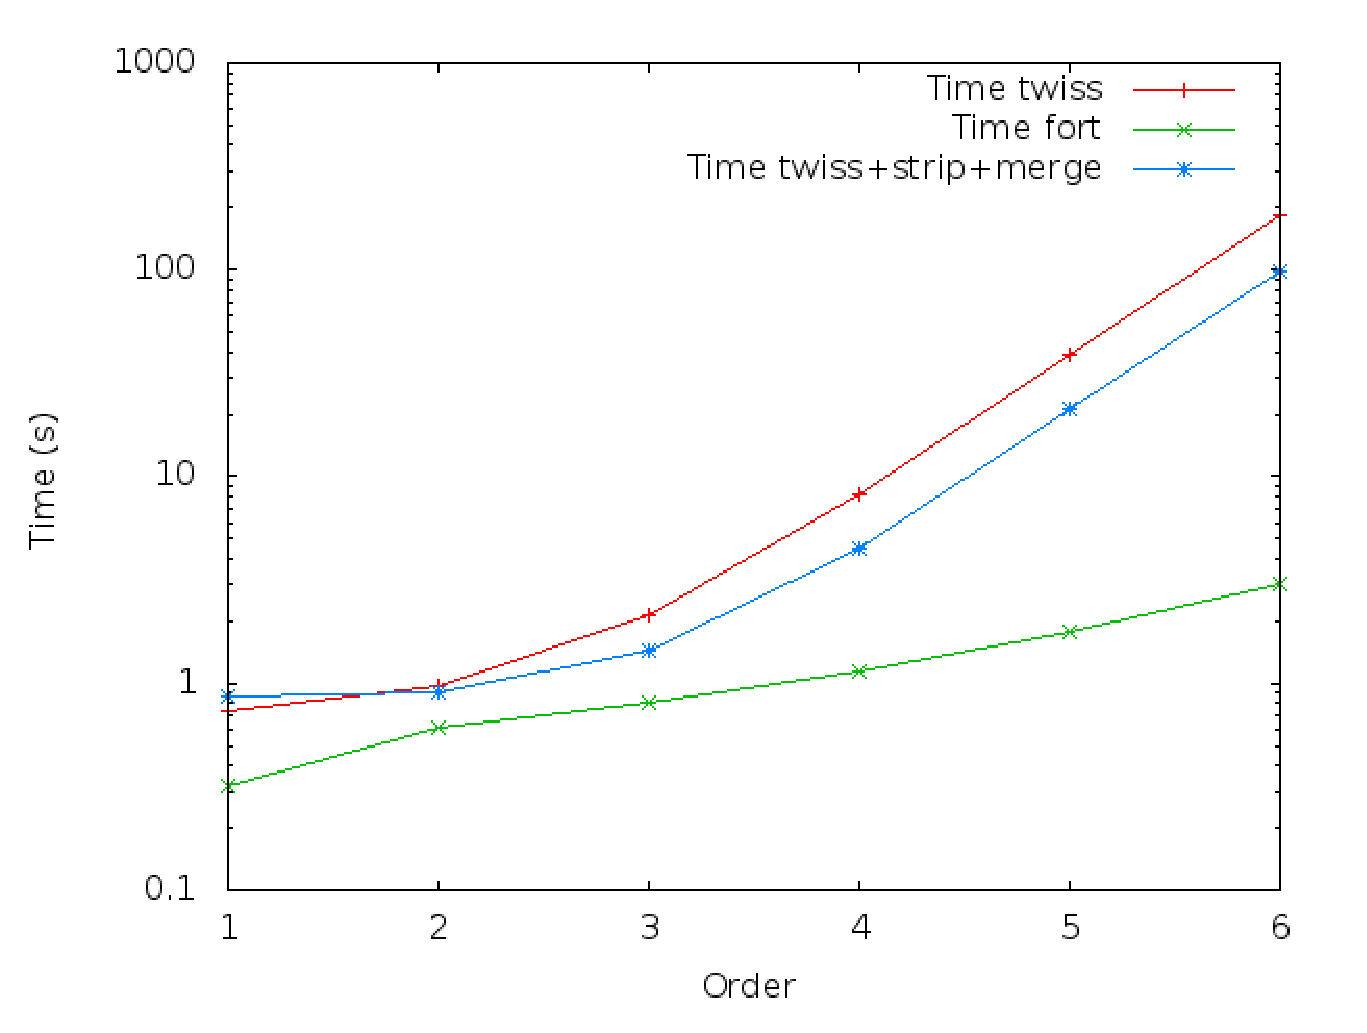
\includegraphics[width=0.8\columnwidth]{imgs/time.eps}
  \caption{Time taken to calculate the sigmas}
  \label{time}
\end{figure}

Figure~\ref{time} shows the time taken by different approaches. The
\textbf{red} line shows the time taken to generate the \textit{twiss}
file through MAD-X, then generating the map with pytpsa and finally
calculating the sigmas. The \textbf{green} line is the time that takes
to generate the \textit{fort.18} with MAD-X plus the time taken by
\textsc{MAPCLASS2} to calculate the sigmas. The \textbf{blue} line is
the time taken to generate the \textit{twiss} file by MAD-X plus the
time taken by \textsc{MAPCLASS2} to strip the line from superfluous
elements and merge the adjacent ones that have the same configuration, then
calculate the map and finally the sigmas. We can see that
although \textsc{MAPCLASS2} gets increasingly slower than PTC as the order is
incremented it is reasonably fast up to order 4, particularly if we consider
the constant gain in time offered by stripping and merging the line.

Further improvements can be obtained by avoiding to generate approximated map
for each element and combine them, but rather directly generate the
composition by using the map resulting from the previous step (instead of the
defaultMap), in analogy of what a tracking code does by passing the final
condition of the previous element as the initial conditions of the next
element. For the first step the initial map is genenerated by the initial
conditions of the orbit plus an identity (defaultMap), which represents a
variation that is kept at lowest order throughout the calculations along the
line.

\subsection{Accuracy}
\label{sec:accuracy}

The accuracy at calculating the map for a given element has been
measured. To do this comparisons between each of the implemented
elements and the corresponding MAD-X PTC generated map were made.

In particular the degradation of the results by increasing the length
of each element was analysed. As expected, for high order elements the
$\chi^2$ error between MAD-X PTC and \textsc{MAPCLASS2} increases
sharply for lengths greater than 5 meters.

See the figures in Appendix~\ref{ap:fig}.

Comparisons of the sigma calculations by \textsc{MAPCLASS2} and
\textsc{MAD-X PTC} have also been made. Figure~\ref{dsigma} shows the
percentage difference of the \textsc{MAPCLASS2} and \textsc{MAD-X PTC}
sigmas for the final focus system. Figure~\ref{dsigma+s+m} shows the
same except that the stripLine() and mergeElems() methods had been
applied to the twiss2 object before generating the map.

\begin{figure}[!hbt]
  \centering
  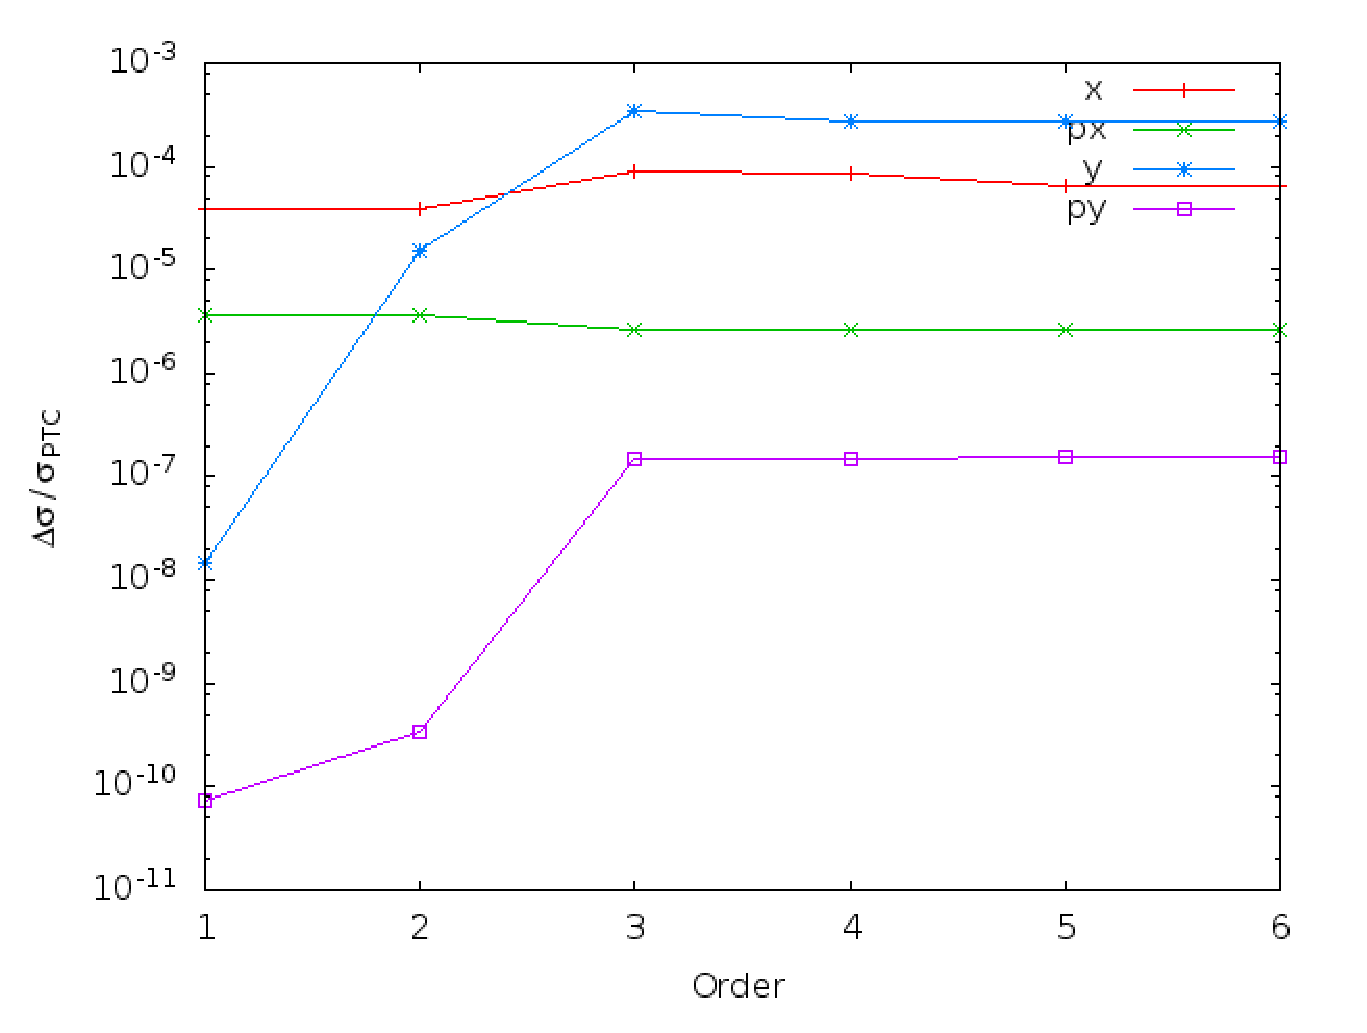
\includegraphics[width=0.8\columnwidth]{imgs/dsigma.eps}
  \caption{Percentage difference of the MAPCLASS2 and MAD-X PTC sigmas}
  \label{dsigma}
\end{figure}

\begin{figure}[!hbt]
  \centering
  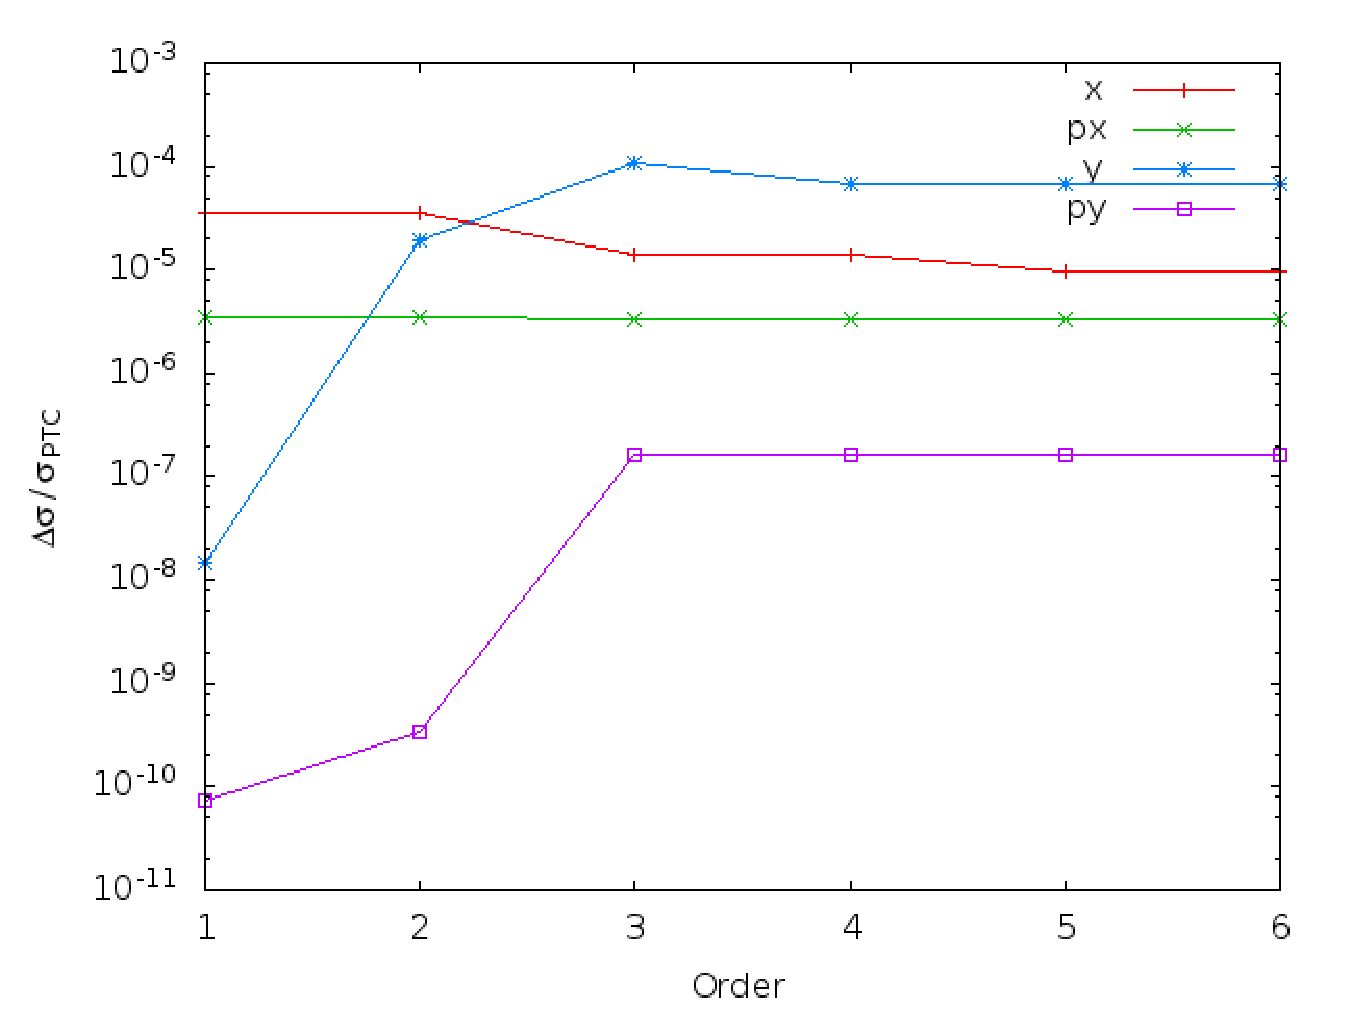
\includegraphics[width=0.8\columnwidth]{imgs/dsigma+strip+merge.eps}
  \caption{Percentage difference of the sigmas with the line stripped
    and merged}
  \label{dsigma+s+m}
\end{figure}

\subsection{Algebra}
% Alternative library - sympy
The entire project utilises the library \textbf{pytpsa} for algebraic
purposes. This means that for any operation within the transport maps
or elsewhere the limitations of the library have to be taken into
account.

\textbf{pytpsa} takes a very simple but elegant solution to represent
polynomials and to operate with them. In addition, by representing quantities
as multivariate polynomials and performing trunctation at a specified order
for each elementary operation, it return machine-precision Taylor expansions
of the user expressions. Special function are like sqrt, sin, asin and so on
are implemented by Taylor expansion, derivative composition rules, Newton
methods, such that they return machine-precision correct results up to the
desired order. Since the library does not support symbolic manimulation like
simplifications or limits, differentiable expressions composed by non
differentiable parts still diverge. In this context alternative formulation of
the expressions should be used.

Python alternatives to \textbf{pytsa} for what concerns the manipulation of
polynomials exists (SymPy~\cite{sympy}, Sage~\cite{sagemath}), although the
truncation rules and special functions needs to be programmed.

Some patches have been suggested in order to speed-up the library.  After
making a quick profiling upon the creation of the map for the FFS it is easy
to conclude that the main bottleneck is the \texttt{fmulpol} method as seen in
Figure~\ref{profiling}.

\begin{figure}[!hbt]
  \centering
  \includegraphics[width=\columnwidth]{imgs/profiling.eps}
  \caption{Profiling the creation of the FFS map}
  \label{profiling}
\end{figure}

One proposed cause for this is \texttt{tuple([l+m for l,m in zip(i,j)])}
within that method. The only obvious line of attack is to redo the low-level
stuff in C, in particular the arithmetic operations. For instance, the line
above takes 1$\mu s$ for 6 long exponents, while adding 6 integers should take
20ns, so there is a factor 50 to gain there. This is detailed in greater
length in the \textit{README} file of the project.

Changing the entire structure of \textsc{MAPCLASS2} to use this library,
however, is non-trivial and it would take a considerable amount of time and
effort. At this point there are not enough drawbacks to push in this direction
to consider attempting this.

\section*{Acknowledgements}
Thanks Oscar Roberto Blanco for contributing to this report by being
the first user of \textsc{MAPCLASS2} and Hector Garc\'ia for his
guidance during the development of the software.

\begin{thebibliography}{9}   % Use for 1-9 reference

\bibitem{mapclass} R.~Tom\'as, AB-Note-2006-017, MAPCLASS: a code to
  optimize high order aberrations.
%
\bibitem{madx} http://mad.web.cern.ch/mad/
%
\bibitem{pytpsa} https://github.com/rdemaria/pytpsa
%
\bibitem{python} http://www.python.org/
%
\bibitem{numpy} http://numpy.scipy.org/
%
\bibitem{lxplus} http://plus.web.cern.ch/plus/
%
\bibitem{afs}
  http://services-old.web.cern.ch/services-old/afs/afsguide.html
%
\bibitem{git} http://git-scm.com/
%
\bibitem{sphinx} http://sphinx.pocoo.org/
%
\bibitem{oide} K. Oide, Phys. Rev. Lett. 61, 1713 - 1715 (1988).
%
\bibitem{sands} M. Sands, Emittance Growth From Radiation
  Fluctuations, Report SLAC/AP-47 (1985).
%
\bibitem{geo} E.~Forest, KEK Preprint 2005-107 (2006), page 55,
  equation 124.
%
\bibitem{esave} http://mad.web.cern.ch/mad/madx.old/error/error\_save.html
%
\bibitem{sympy}
  http://sympy.org/en/index.html

\bibitem{sagemath}
  http://www.sagemath.org/

\end{thebibliography}

\clearpage
\appendix
\section{Appendix}

\subsection{Formulae}
\subsubsection{Transport Matrices}
\label{ap:trans1}
\textbf{Drift space}

\[
M
=
\begin{bmatrix}
1 & \frac{L}{1+\delta} & 0 & 0 & 0 & 0 \\[0.3em]
0 & 1 & 0 & 0 & 0 & 0 \\[0.3em]
0 & 0 & 1 & \frac{L}{1+\delta} & 0 & 0 \\[0.3em]
0 & 0 & 0 & 1 & 0 & 0 \\[0.3em]
0 & 0 & 0 & 0 & 1 & 0 \\[0.3em]
0 & 0 & 0 & 0 & 0 & 1
\end{bmatrix}
\]
\\\\
\textbf{Dipole sector magnet} $(\theta = \frac{ANGLE}{\sqrt{1+\delta}},\:
\rho = \frac{l}{ANGLE})$

\[
M
=
\begin{bmatrix}
\cos(\theta) & \rho \sin(\theta) & 0 & 0 & \rho(1-\cos(\theta)) & 0
\\[0.3em]
-\frac{1}{\rho}\sin(\theta) & \cos(\theta) & 0 & 0 &
\sqrt{1+\delta}\sin(\theta) & 0 \\[0.3em]
0 & 0 & 1 & \frac{L}{1+\delta} & 0 & 0 \\[0.3em]
0 & 0 & 0 & 1 & 0 & 0 \\[0.3em]
0 & 0 & 0 & 0 & 1 & 0 \\[0.3em]
0 & 0 & 0 & 0 & 0 & 1
\end{bmatrix}
\]
\\\\
\textbf{Focusing Quadrupole} $(K =|\frac{\frac{K1L}{L}}{1+\delta}|)$

\[
M
=
\begin{bmatrix}
\cos(L\sqrt{K}) & \frac{1}{\sqrt{K}} \frac{\sin(L\sqrt{K})}{1+\delta} & 0 & 0
& 0 & 0\\[0.3em]
-\sqrt{K}\sin(L\sqrt{K})(1+\delta) & \cos(L\sqrt{K}) & 0 & 0 & 0 & 0
\\[0.3em]
0 & 0 & \cosh(L\sqrt{K}) & \frac{1}{\sqrt{K}}\frac{\sinh(L\sqrt{K}}{1+\delta}
& 0 & 0 \\[0.3em]
0 & 0 & \sqrt{K}\sinh(L\sqrt{K})(1+\delta) & \cosh(L\sqrt{K}) & 0 & 0
\\[0.3em]
0 & 0 & 0 & 0 & 1 & 0 \\[0.3em]
0 & 0 & 0 & 0 & 0 & 1
\end{bmatrix}
\]
\newpage
\textbf{Defocusing Quadrupole} $(K =|\frac{\frac{K1L}{L}}{1+\delta}|)$

\[
M
=
\begin{bmatrix}
\cosh(L\sqrt{K}) & \frac{1}{\sqrt{K}}\frac{\sinh(L\sqrt{K}}{1+\delta} & 0 & 0
& 0 & 0\\[0.3em]
\sqrt{K}\sinh(L\sqrt{K})(1+\delta) & \cosh(L\sqrt{K}) & 0 & 0 & 0 & 0
\\[0.3em]
0 & 0 & \cos(L\sqrt{K}) & \frac{1}{\sqrt{K}} \frac{\sin(L\sqrt{K})}{1+\delta}
& 0 & 0 \\[0.3em]
0 & 0 & -\sqrt{K}\sin(L\sqrt{K})(1+\delta) & \cos(L\sqrt{K}) & 0 & 0
\\[0.3em]
0 & 0 & 0 & 0 & 1 & 0 \\[0.3em]
0 & 0 & 0 & 0 & 0 & 1
\end{bmatrix}
\]

\subsubsection{Transport Maps}
\label{ap:trans2}
\textbf{Thin multipoles}
\[
px = px + \sum_{n=1}^{4} -\Re \begin{Bmatrix}\frac{1}{n!} (x +
  jy)^n\end{Bmatrix} K_n L\\[0.4em]
\]
\[
py = py + \sum_{n=1}^{4} \Im \begin{Bmatrix}\frac{1}{n!} (x +
  jy)^n\end{Bmatrix} K_n L
\]

where j is the imaginary unit.
\\

\textbf{Thick multipoles}

Where the kick for each of the 6 slices are given by:
\[
\frac{c_i}{k} = \left(\frac{41}{840}, \frac{9}{35}, \frac{9}{280},
\frac{34}{105}, \frac{9}{280}, \frac{9}{35}, \frac{41}{840} \right)
\]

as described in~\cite{geo}.

\subsubsection{Transformation of $\alpha, \beta, \gamma$}
\label{ap:beta}
\[
\begin{bmatrix}
\beta \\[0.3em]
\alpha \\[0.3em]
\gamma
\end{bmatrix}
=
\begin{bmatrix}
C^2 & 2SC & S^2 \\[0.3em]
-CC' & SC' + S'C & -SS'\\[0.3em]
C'^2 & -2S'C' & S'^2
\end{bmatrix}
\begin{bmatrix}
\beta_0 \\[0.3em]
\alpha_0 \\[0.3em]
\gamma_0
\end{bmatrix}
\]

where C, S, C' and S' are elements of the transport matrices such
that:
\[
\begin{bmatrix}
x \\[0.3em]
x'
\end{bmatrix}
=
\begin{bmatrix}
C & S \\[0.3em]
C' & S'
\end{bmatrix}
\begin{bmatrix}
x_0 \\[0.3em]
x'_0
\end{bmatrix}
\]

\subsubsection{Dispersion Function}
\label{ap:disp}
\[
\begin{bmatrix}
\eta \\[0.3em]
\eta' \\[0.3em]
1
\end{bmatrix}
=
\begin{bmatrix}
C & S & D \\[0.3em]
C' & S' & D'\\[0.3em]
0 & 0 & 1
\end{bmatrix}
\begin{bmatrix}
\eta_0 \\[0.3em]
\eta'_0 \\[0.3em]
1
\end{bmatrix}
\]
where D and D' correspond to the dispersion trajectory part of the
transport matrix and $\eta$ and $\eta'$ refer to the dispersions D and
DP respectively.

\subsubsection{Phase, $\phi$}
\label{ap:phase}
\[
\begin{bmatrix}
C & S\\[0.3em]
C' & S'
\end{bmatrix}
=
\begin{bmatrix}
\sqrt{\frac{\beta}{\beta_o}}(\cos{\Delta \phi} + \alpha_o \sin{\Delta
  \phi}) & \sqrt{\beta \beta_o} \sin{\Delta \phi}\\[0.3em]
\frac{1}{\sqrt{\beta \beta_o}}((\alpha_o - \alpha)\cos{\Delta \phi} -
(1+ \alpha \alpha_o)\sin{\Delta \phi}) &
\sqrt{\frac{\beta_o}{\beta}}(\cos{\Delta \phi} - \alpha \sin{\Delta
  \phi})
\end{bmatrix}
\]
\\\\
with $\Delta \phi = \phi (s) - \phi (s_o)$.

\begin{equation}
\label{ph:sin}
\sin{\Delta \phi} = \frac{S}{\sqrt{\beta \beta_o}}
\end{equation}
\begin{equation}
\label{ph:cos}
\cos{\Delta \phi} = \sqrt{\frac{\beta_o}{\beta}}C - \alpha_o
\frac{S}{\sqrt{\beta \beta_o}}
\end{equation}

Using results for C and S from  the transport matrices in
(\ref{ph:sin}) and (\ref{ph:cos}):

\[
\phi(s) = \arctan(\sin{\Delta \phi},\cos{\Delta
\phi})/2\pi + \phi (s_o)
\]

\subsubsection{Natural Chromaticity}
\label{ap:natchrom}
$\xi_y = (X_{y,00101}X_{y,00101} \frac{\beta_{y0}}{\beta^*_y} +
X_{y,00011}X_{y,00011} \frac{1}{\beta^*_y \beta_{y0}} )$

\subsubsection{Chromaticity}
\label{ap:chrom}
$\xi = -\frac{1}{4\pi} \int \beta K ds$

\subsubsection{$\mathcal{H}$ Function}
\label{ap:h}
$\mathcal{H}(s) = \gamma \eta^2 + 2 \alpha \eta\eta' + \beta \eta'^2$

\subsubsection{Synchrotron Radiation: Oide Effect}
\label{ap:oide}
$\Delta \sigma^2_{OIDE} = \frac{110}{3\sqrt{6\pi}} r_e \lambda_e
\gamma^5 F(K_q,L_q,l^*) (\frac{\epsilon_y}{\beta^*_y})^\frac{5}{2}$
\\\\
where
\[
F(K_q,L_q,l^*) = \int\limits_0^{\sqrt{K_q}L_q} |\sin(y) +
\sqrt{K_q}l^* \cos(y)|^3 \left[\int\limits_0^y (\sin(x) + \sqrt{K_q}l^*
  \cos(x))^2 dx\right]^2 dy
\]

$r_e$ is the radius of an electron, $\lambda_e$ is the Compton
wavelength, $\gamma = \frac{E}{E_0}$ is the Lorentz factor for an
electron in the CLIC, $L_q$ is the length of the final quadrupole,
$K_q$ is its strength, $l^*$ is the length of the drift space between
the final quadrupole and the IP, $\epsilon_y$ is the emittance and
$\beta_y^*$ is the design $\beta$.

\subsubsection{Synchrotron Radiation: Bends}
\label{ap:bends}
$\Delta \sigma^2_{BENDS} = C_2 \beta_L E_o^5
\int\limits_0^s G(s)^3 \mathcal{H}(s) \cos(\Phi(s))^2 ds$,
\\\\
where
\\\\
$C_2 = \frac{55}{24 \sqrt{3}} \frac{r_e \hbar c}{(mc^2)^6} = 4.13
\times 10^{-11} m^2(GeV)^{-5}$,
\\\\
$G(s) = \frac{1}{\rho (s)}$,
\\\\
$\Phi(s) = \phi(L) - \phi(s) + \alpha(s)$, where $\alpha(s) =
\arctan(\frac{\beta'}{2} - \frac{\beta \eta'}{\eta})$
\\\\
$\beta_L$ is the design $\beta$ and $E_o$ is the average energy.

\newpage
\subsection{Required MAD-X Columns}
\label{ap:columns}
\texttt{NAME, KEYWORD, S, L, BETX, BETY, ALFX, ALFY, MUX, MUY, DX, DPX,
  DY, DPY, ANGLE, K1L, K2L, K3L, K4L} \footnote{Subject to change. The
columns listed here are the ones required at the time this note was published}


\subsection{Figures}
\label{ap:fig}

\begin{figure}[!h]
  \centering
  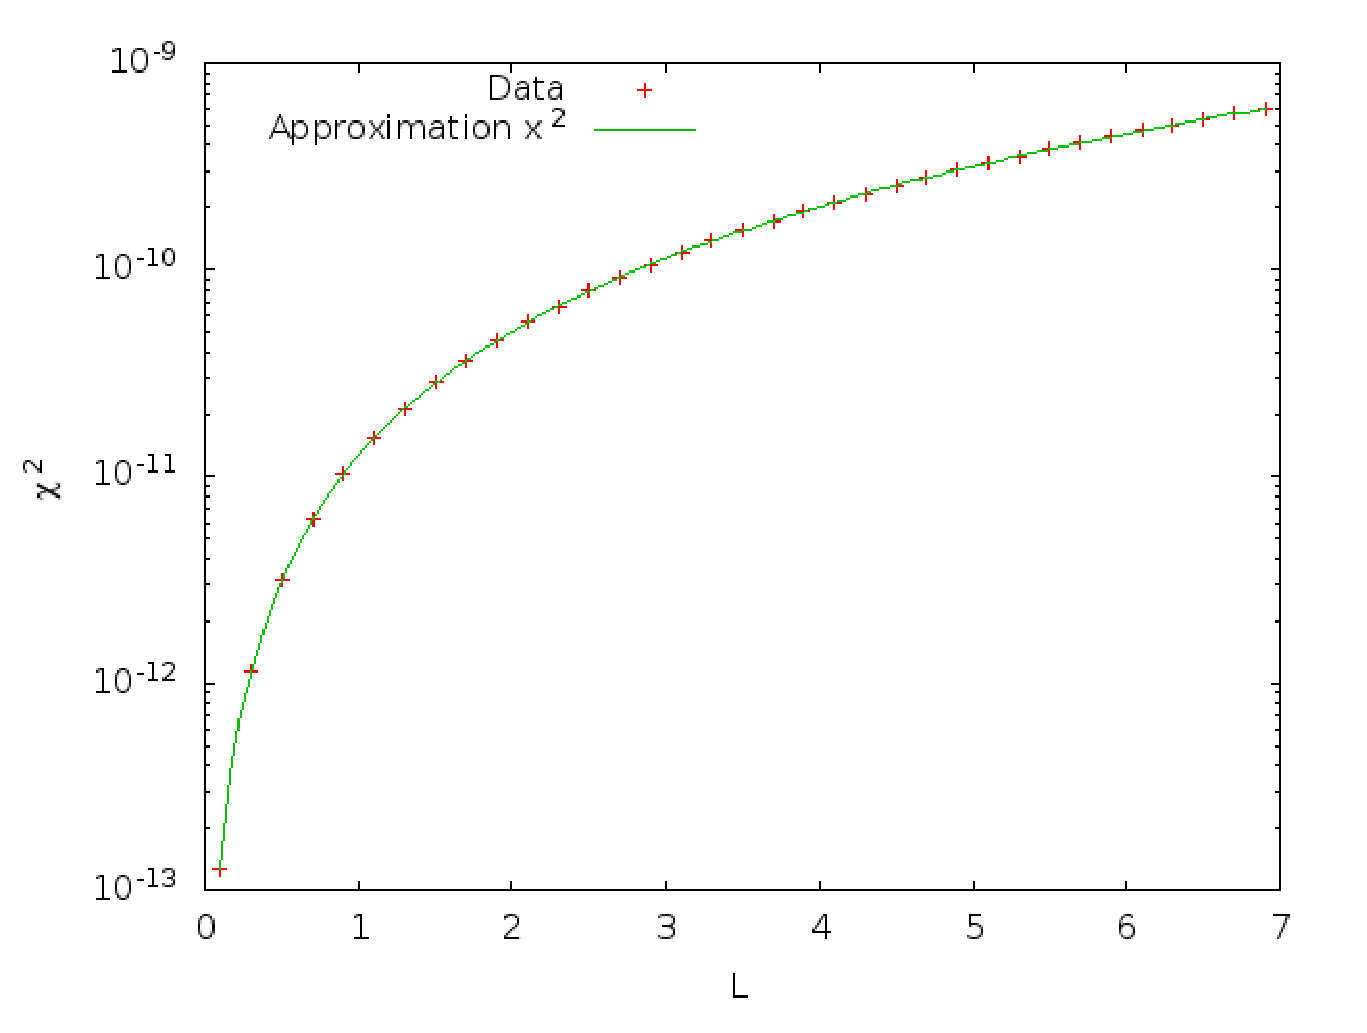
\includegraphics[width=0.8\columnwidth]{imgs/dr.eps}
  \caption{Drift space}
\end{figure}

\begin{figure}
  \centering
  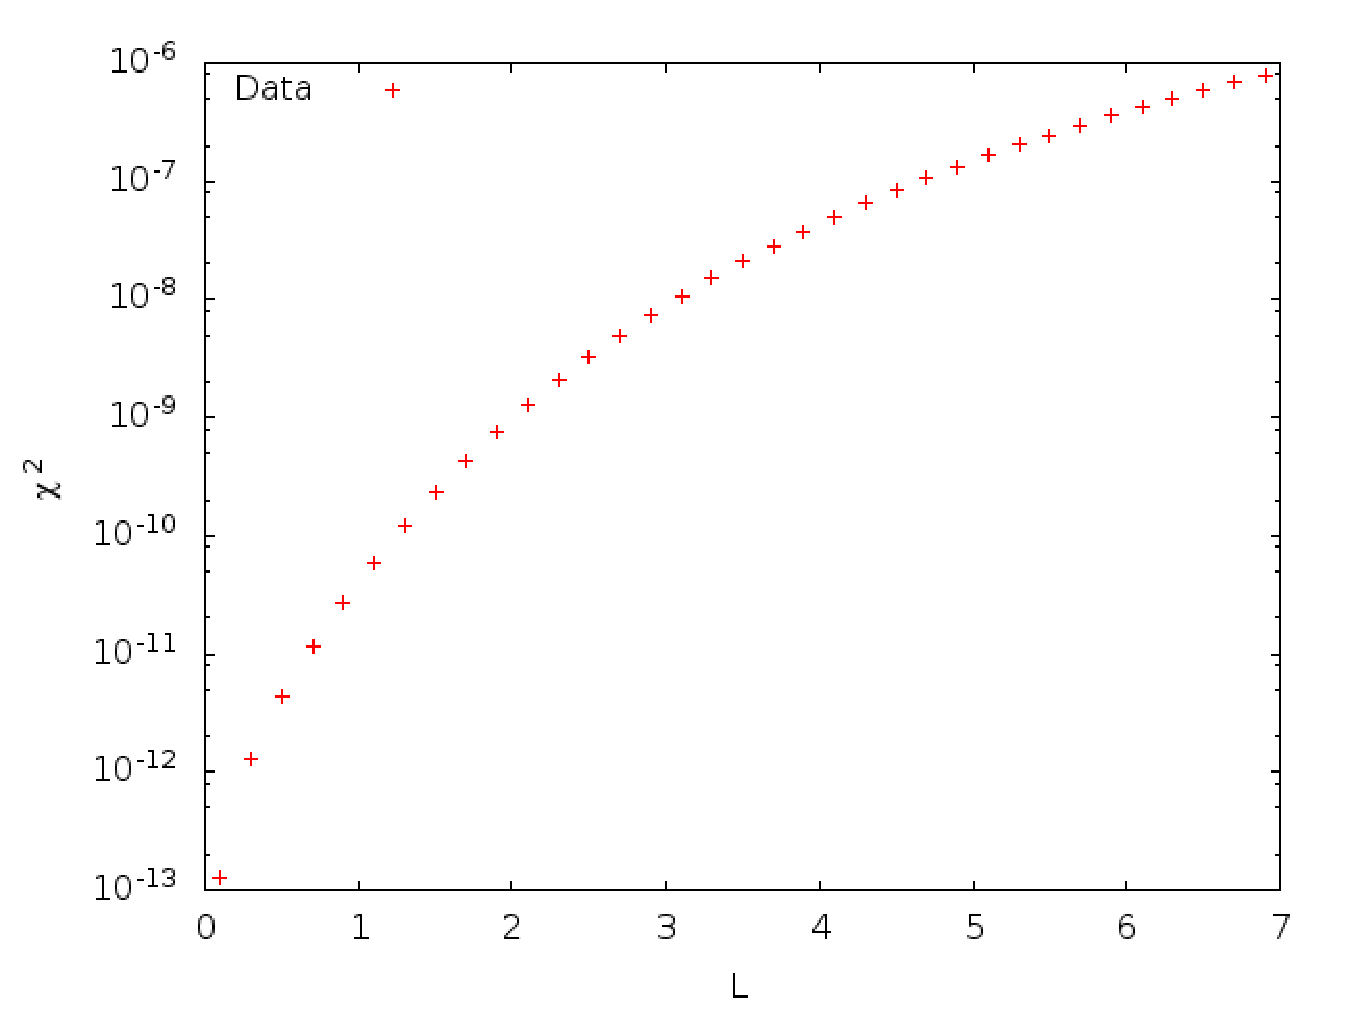
\includegraphics[width=0.8\columnwidth]{imgs/di.eps}
  \caption{Dipole ($ANGLE = L\times 5^{\circ}$)}
\end{figure}

\begin{figure}
  \centering
  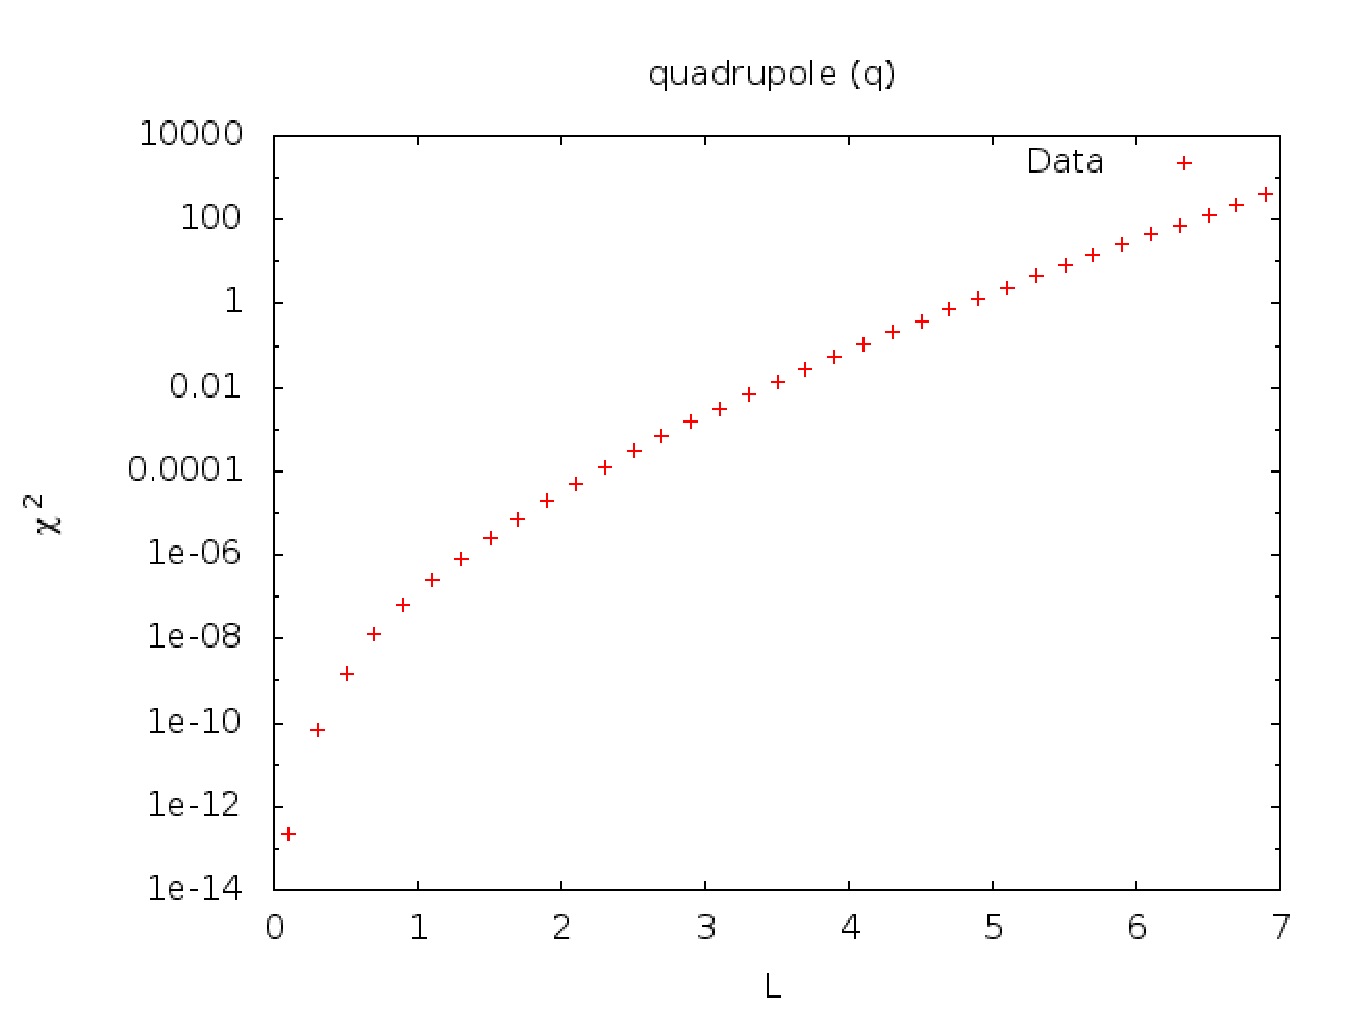
\includegraphics[width=0.8\columnwidth]{imgs/q.eps}
  \caption{Quadrupole (K = 0.5$m^{-2}$)}
\end{figure}

\begin{figure}
  \centering
  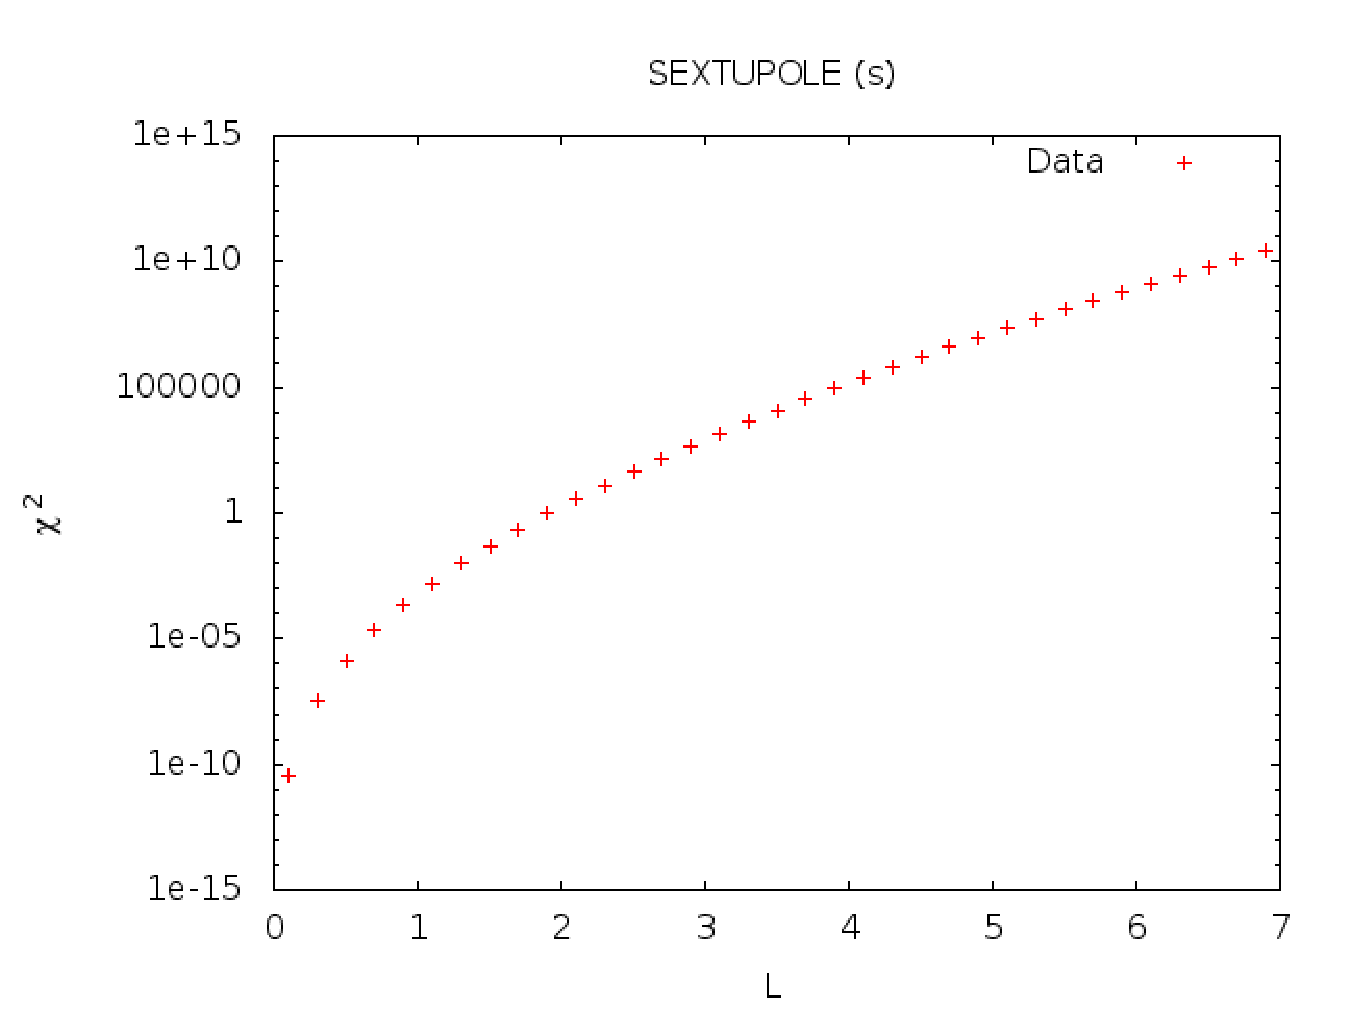
\includegraphics[width=0.8\columnwidth]{imgs/s.eps}
  \caption{Sextupole (K = 0.5$m^{-3}$)}
\end{figure}

\begin{figure}
  \centering
  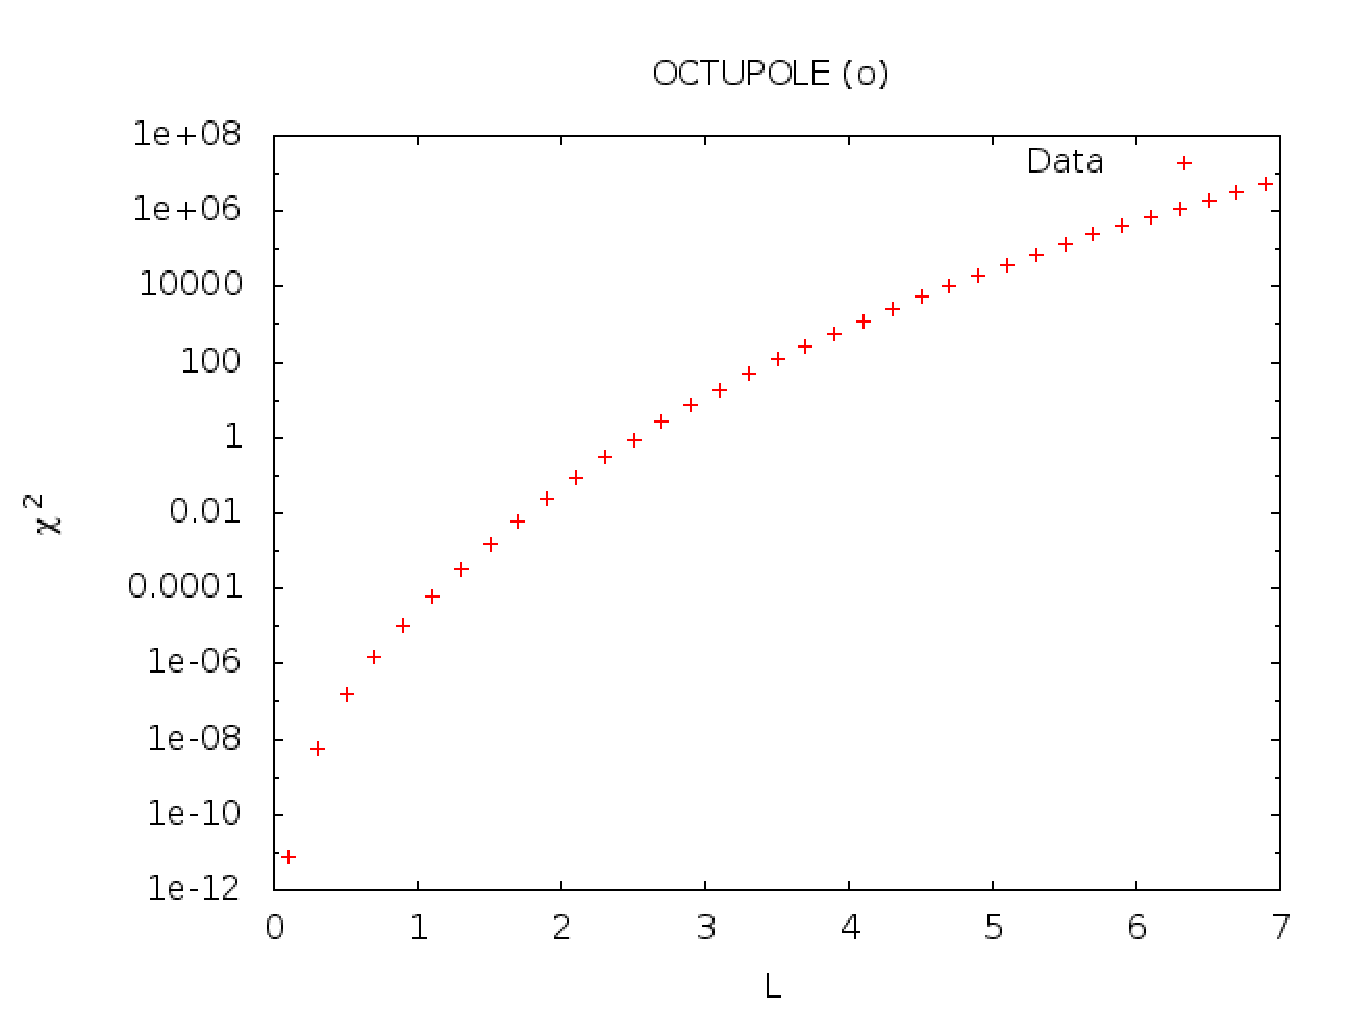
\includegraphics[width=0.8\columnwidth]{imgs/o.eps}
  \caption{Octupole (K = 0.4$m^{-4}$)}
\end{figure}

\end{document}
